\section{Data}
\label{sec:data}
\begin{table}[ht]
\centering
{%
\begin{tabular}{lrr}
\toprule
 & Adj Close & Log Return \\
\midrule
count & 900.00 & 900.00 \\
mean & 841.30 & 0.01 \\
std & 1160.66 & 0.04 \\
min & 16.79 & -0.25 \\
25\% & 89.10 & -0.02 \\
50\% & 260.11 & 0.01 \\
75\% & 1247.29 & 0.03 \\
max & 5969.34 & 0.15 \\
\bottomrule
\end{tabular}
}
\caption{Summary statistics of the S\&P 500 monthly log returns. Data is sourced from Yahoo Finance \citep{yahoo_finance_gspc}.}
\label{tab:sp500_returns_summary}
\end{table}
We use Python \citep{python3}, Pandas \citep{reback2020pandas}, NumPy \citep{harris2020array}, Statsmodels \citep{seabold2010statsmodels}, and Arch \citep{sheppard2024arch} to analyze S\&P 500 price data from Yahoo Finance \citep{yahoo_finance_gspc} and the Fama-French 3-factor data library \citep{french_website}.
Yahoo Finance provides daily price data of the S\&P 500 which we resample to monthly returns for the period 1950 - 2024. We get monthly log returns by taking the
difference of the log of the adjusted close price of the S\&P 500 for each month (Figure~\ref{fig:sp500_returns}, Table~\ref{tab:sp500_returns_summary}). Our time series starts in 1950
based on the premise that the market prior to this was not as sophisticated, and is not illustrative for the purposes of this analysis of market efficiency and value spreads. \citep{asness_2024} justifies this using the 
instability of value spreads prior to 1950. We use the log of the adjusted close price to account for stock splits and dividends, and to make the returns more comparable over time.
We use Matplotlib for plotting \citep{Hunter2007}.
\begin{figure}[h!]
    \centering
    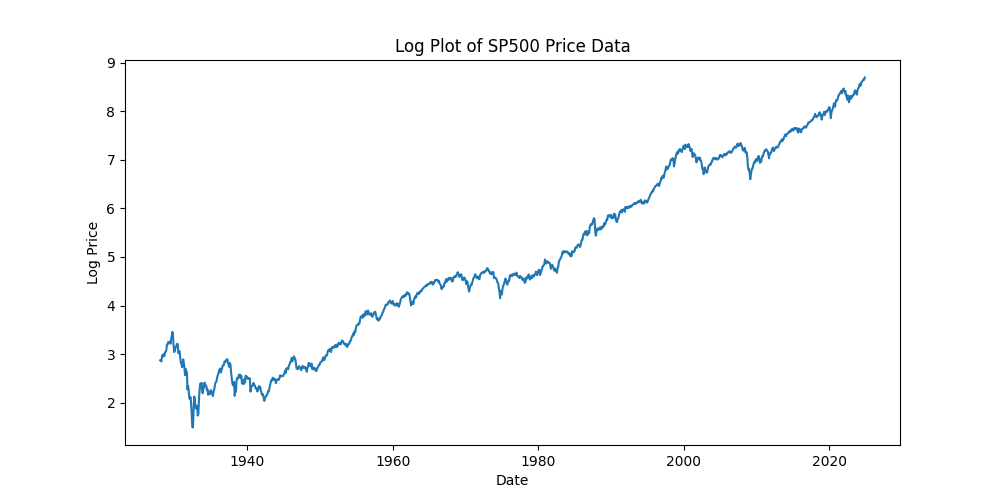
\includegraphics[width=1\textwidth]{../figs/SP500_Log_Price.png}
    \caption{The S\&P 500 time series 1950 - 2024. We use log-prices, the log of the adjusted and observe this plot, noticing nothing unusual.}
    \label{fig:sp500_returns}
\end{figure}

\subsection{Cumulative Log Returns}
\begin{table}[ht]
\centering
\resizebox{\textwidth}{!}{%
\begin{tabular}{lrrrrrrr}
\toprule
Date & Cum Log Return 1 & Cum Log Return 2 & Cum Log Return 3 & ... & Cum Log Return 34 & Cum Log Return 35 & Cum Log Return 36 \\
\midrule
1950-01-01 & 0.0154 & 0.0253 & 0.0293 & ... & 0.379 & 0.424 & 0.459 \\
1950-02-01 & 0.0100 & 0.0140 & 0.0520 & ... & 0.409 & 0.444 & 0.436 \\
1950-03-01 & 0.00412 & 0.0421 & 0.0867 & ... & 0.434 & 0.427 & 0.408 \\
1950-04-01 & 0.0380 & 0.0827 & 0.0229 & ... & 0.422 & 0.404 & 0.380 \\
1950-05-01 & 0.0446 & -0.0151 & -0.00672 & ... & 0.366 & 0.342 & 0.315 \\
\bottomrule
\end{tabular}
}
\caption{Cumulative log S\&P500 return periods for each month. Each column represents the cumulative log return for a given period starting 
at the row index, and ending $t$ months ahead.}
\label{tab:cumulative_log_returns}
\end{table}

The unbiasedness regression require windows of cumulative returns. For any month $t$, we get every forward month's returns up to T months.
By taking expanding window sums of the columns of log returns, we get a cumulative log returns matrix (Table~\ref{tab:cumulative_log_returns}).

\begin{table}[ht]
\centering
{%
\begin{tabular}{lr}
\toprule
 & Value Spread \\
\midrule
count & 897.00 \\
mean & 4.89 \\
std & 1.33 \\
min & 3.29 \\
25\% & 4.06 \\
50\% & 4.56 \\
75\% & 5.36 \\
max & 9.96 \\
\bottomrule
\end{tabular}
}
\caption{Summary statistics of the value spread time series. The value spread is the ratio of the average book-to-market of the most expensive 30\% portfolio to the average book-to-market of the portfolio of the cheapest 30\% of stock portfolio. Data from French's Website \citep{french_website}.}
\label{tab:value_spread_summary}
\end{table}
\subsection{The Value Spread}
The value spread is a ratio of the average book-to-market of the most expensive 30\% portfolio to the average book-to-market of the portfolio of the cheapest 30\% of stock portfolio, as per \citet{fama_french_1993}.
To construct this measure we use Kenneth French's data library \citep{french_website} (Figure~\ref{fig:value_spread}, Table~\ref{tab:value_spread_summary}). 
Using French's 3x2 sort on book-to-market and market equity, we get the monthly market value weighted average of the book-to-value of the portfolio of the 30\% most expensive large-cap stocks and the portfolio of the 30\% cheapest large-cap stocks.
Dividing the two averages represents how much more expensive the expensive stocks are compared to the cheap stocks.

\begin{figure}[h!]
    \centering
    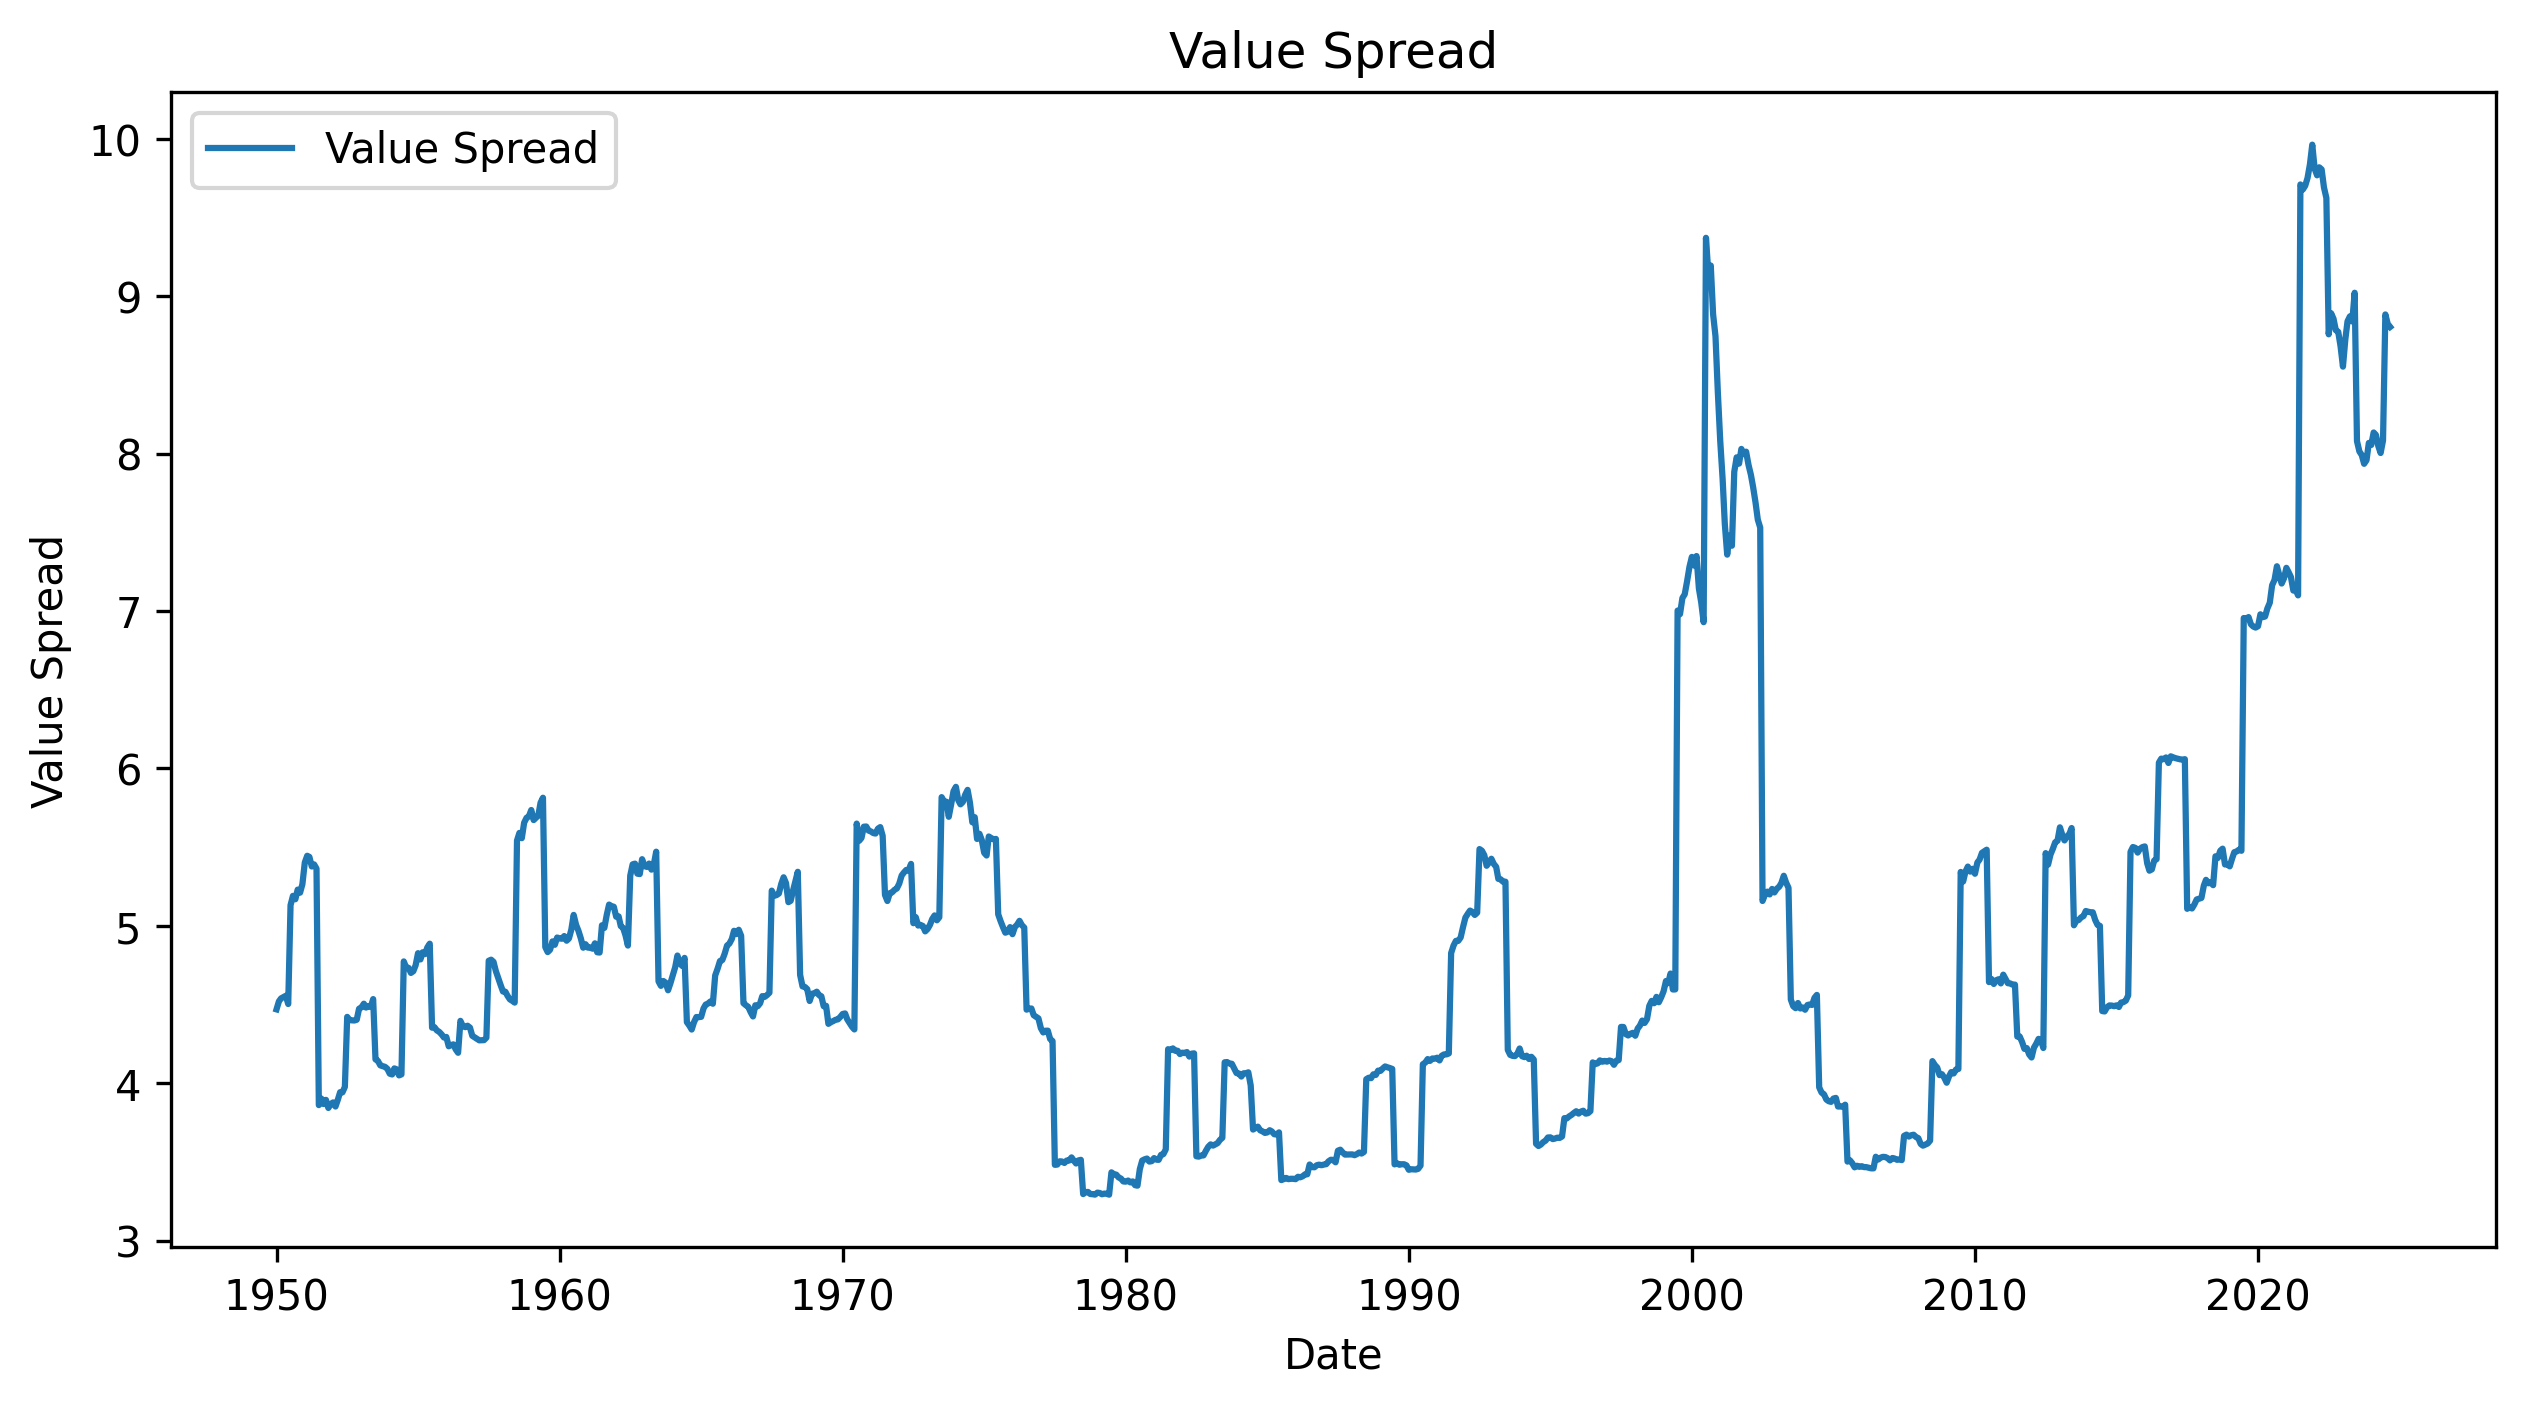
\includegraphics[width=1\textwidth]{../figs/Value_Spread.png}
    \caption{The value spread time series 1950 - 2024. \citet{asness_2024} argues the widening spread in the last decade is due to increasing market inefficiency.}
    \label{fig:value_spread}
\end{figure}

\subsection{Measurement}
We use cumulative log returns of the S\&P 500 because every cumulative return window represents the information content of that time period. Partial cumulative return
windows demonstrate the information content up to a point in the entire period. Using the subsets of a cumulative window period together, we get an idea of the
information flows within the wider cumulative period window. We use the S\&P 500 because its returns are more representative of the average market information ability
than the returns for a single firm, which would be subject to idiosyncratic shocks. The S\&P 500 also represents larger firms, which are heavily observed by market participants, and have well-regulated information flow, 
so should represent the most efficiently priced index. I expand on how these components representing information flow lead to a measure of market inefficiency in Section~\ref{sec:market_efficiency}.